\documentclass[8pt,twocolumn]{article}
\setlength{\columnsep}{15pt}

\usepackage[letterpaper, margin=0.75in]{geometry}

\usepackage{graphicx}
\graphicspath{ {./images/} }

\usepackage{listings}
\usepackage{amsmath}

\usepackage{xcolor}

\usepackage{apacite}
\renewcommand\bibliographytypesize{\small}
\usepackage[hyphens,spaces,obeyspaces]{url}

\newcommand{\ssub}[1]{\bigskip\noindent{\textbf{#1}}\smallskip}
\newcommand{\xssub}[1]{\bigskip\noindent{\small\textbf{#1}}\smallskip}

\title{A Smart Aquatic Control Platform}
\author{Jingwei Dai\\Department of Computer Science\\Earlham College\\Richmond IN, USA\\adai13@earlham.edu\\}
\date{May, 2024}

\begin{document}

\maketitle

\begin{abstract}
The marine aquarium industry has been exploring IoT (Internet of Things) technologies to automate maintenance, yet existing solutions often rely on proprietary Wi-Fi or Bluetooth implementations, hindering the development of reliable hardware. Moreover, these solutions operate within isolated ecosystems, posing integration challenges with established Smart Home platforms like Apple’s HomeKit.

This project explores the latest advancements in IoT connectivity standards, particularly focusing on Thread and its open-source counterpart, OpenThread. Our objective is to establish a Platform leveraging OpenThread that empowers third-party IoT manufacturers to easily build Thread-enabled products for specific applications within large-scale artificial environments, such as aviaries and marine aquariums. In addition, we developed a hardware prototype to showcase distinct advantages of a connected aquatic control system over traditional aquarium setups. Overall, the Platform means to highlight an integrated experience where a focus on ease of access and onboarding, both through the adoption of Thread and HomeKit, enhances the user experience and drives the development of animal-care technologies.
\end{abstract}

\section*{Keywords}

SwiftUI, HomeKit, Beaglebone Black, Thread, OpenThread

\section{Introduction}

The current smart home landscape is dominated by three major platforms: Amazon Alexa, Apple HomeKit, and Google Home, all backed by their respective smart assistants. These define the quintessential frontend user experience, because they are what users directly interact with to control their smart homes. Throughout the 2010s, choosing which platform to stick with was an important decision. The platforms were not interoperable: Alexa, Siri, and Google Assistant spoke totally different languages under the hood, and most smart home products could only be connected to one platform at a time. Over the last few years, tech giants have come together to remedy the situation \shortcite{lackofstandardization}. The result is Matter, an open-source interoperability standard that vows to unite the world of IoT \shortcite{wired}. All three platforms have signed on to fully integrate the Matter application layer in the next few years, which means they will eventually sport the same backend with the only difference being UI/UX. When the transition completes, smart home devices conforming to Matter will work under all platforms without extra tinkering. The eventual engineering product of this project will be fully compatible the Apple HomeKit platform, which already runs on a backend that fully supports Matter \cite{AppleHomekitMatter}.

The platforms, including those that have transitioned to Matter, support multiple connection protocols through which devices talk to the platform backend and each other. As of 2023, there are half a dozen popular protocols in the IoT industry \shortcite{Pradeep}. Major IoT manufacturers Philips and Aqara use ZigBee as the protocol for their entire line of smart home devices \cite{Hue}. ZigBee devices do not talk to the platforms directly. They can only function when a hub is connected to the internet router to act as a relay for communication between themselves and the platform backend, but hubs from some manufacturers are not compatible with competitors' devices. For example, Aqara's ZigBee implementation veers off the standard by an enough amount that third party devices cannot connect to Aqara's hubs.

However, standardization through Matter may solve this fragmentation of technology in the IoT industry. Matter recommends Thread, a relatively new protocol that consolidates the advantages of the most popular connection protocols. With the inclusion of a Thread radio in the iPhone 15 \cite{AppleThreadiPhone15}, we are seeing major effort from industry leaders to promote and facilitate the adoption of this technology.

By employing Thread as the foundational technology, we differentiate ourselves from comparable platforms in the market. Thread provides a robust infrastructure with low-latency, low-bandwidth, and low-power connectivity, establishing a mesh network among connected devices. This enables swift responses to user inputs and ensures platform scalability without compromising performance.

\begin{figure}[!htbp]
    \centering
    \makebox[0pt]{%
    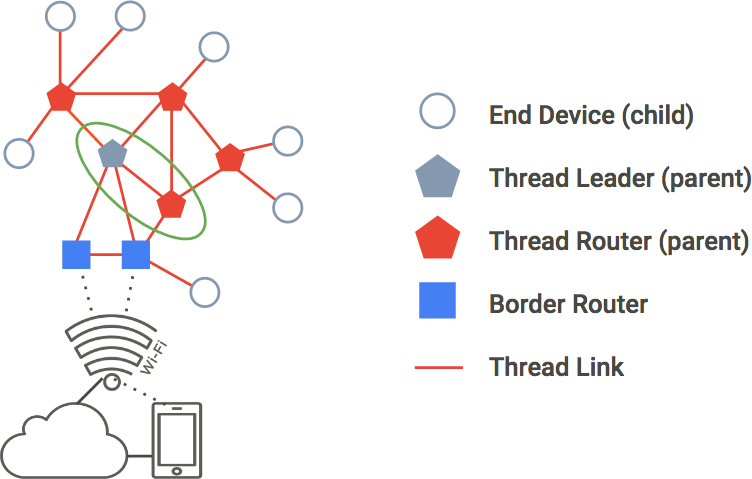
\includegraphics[width=0.9\linewidth]{thread_topo}}
    \caption{Thread Topology \protect\cite{thread_topology}}
\end{figure}

Additionally, Thread devices boasts of a fallback mechanism called Border Routers assumable by all non-battery powered devices. Thread intelligently selects devices to serve as Border Routers, each enabling bidirectional connectivity between the mesh network and the internet. This approach significantly reduces the risk of system-wide shutdown caused by a single device failure. This contrasts with traditional low-latency smart home platforms that rely on a dedicated hub, which introduces a single point of failure capable of crippling the entire system.

Our vision for the Platform extends to serving systems of all sizes, ranging from home reef tanks to industrial coral farms and public aquariums. The integration of remote-controllable devices that establish a scalable mesh network among themselves greatly facilitates the management of these diverse systems, while Thread's fallback mechanism protects artificial ecosystems where stability is of the utmost importance.

In the aquarium industry, a frequent frustration among users of smart devices is the necessity to navigate through the manufacturer's app for even basic tasks. We offer a solution by exposing commonly-used device settings through HomeKit and by giving users the ability to customize which settings are most important to them. This enables users to, for instance, instruct Siri with a single command to activate the spectrum that enhances the color of corals right before the guests' arrival, rather than adjusting various sliders manually. HomeKit is integrated into all iOS devices, ensuring seamless accessibility.

\section{Project Goal}

In this project phase, our aim is to demonstrate the enhanced user experience and effectiveness in aquarium maintenance through an integrated aquatic control system. We've developed an iOS app and a hardware demo utilizing OpenThread's IoT Debian OS. Leveraging the Beaglebone's sensor capabilities, we showcase the potential of a smart home platform within the aquarium industry.

\section{Components}

\begin{figure}[!htbp]
    \centering
    \makebox[0pt]{%
    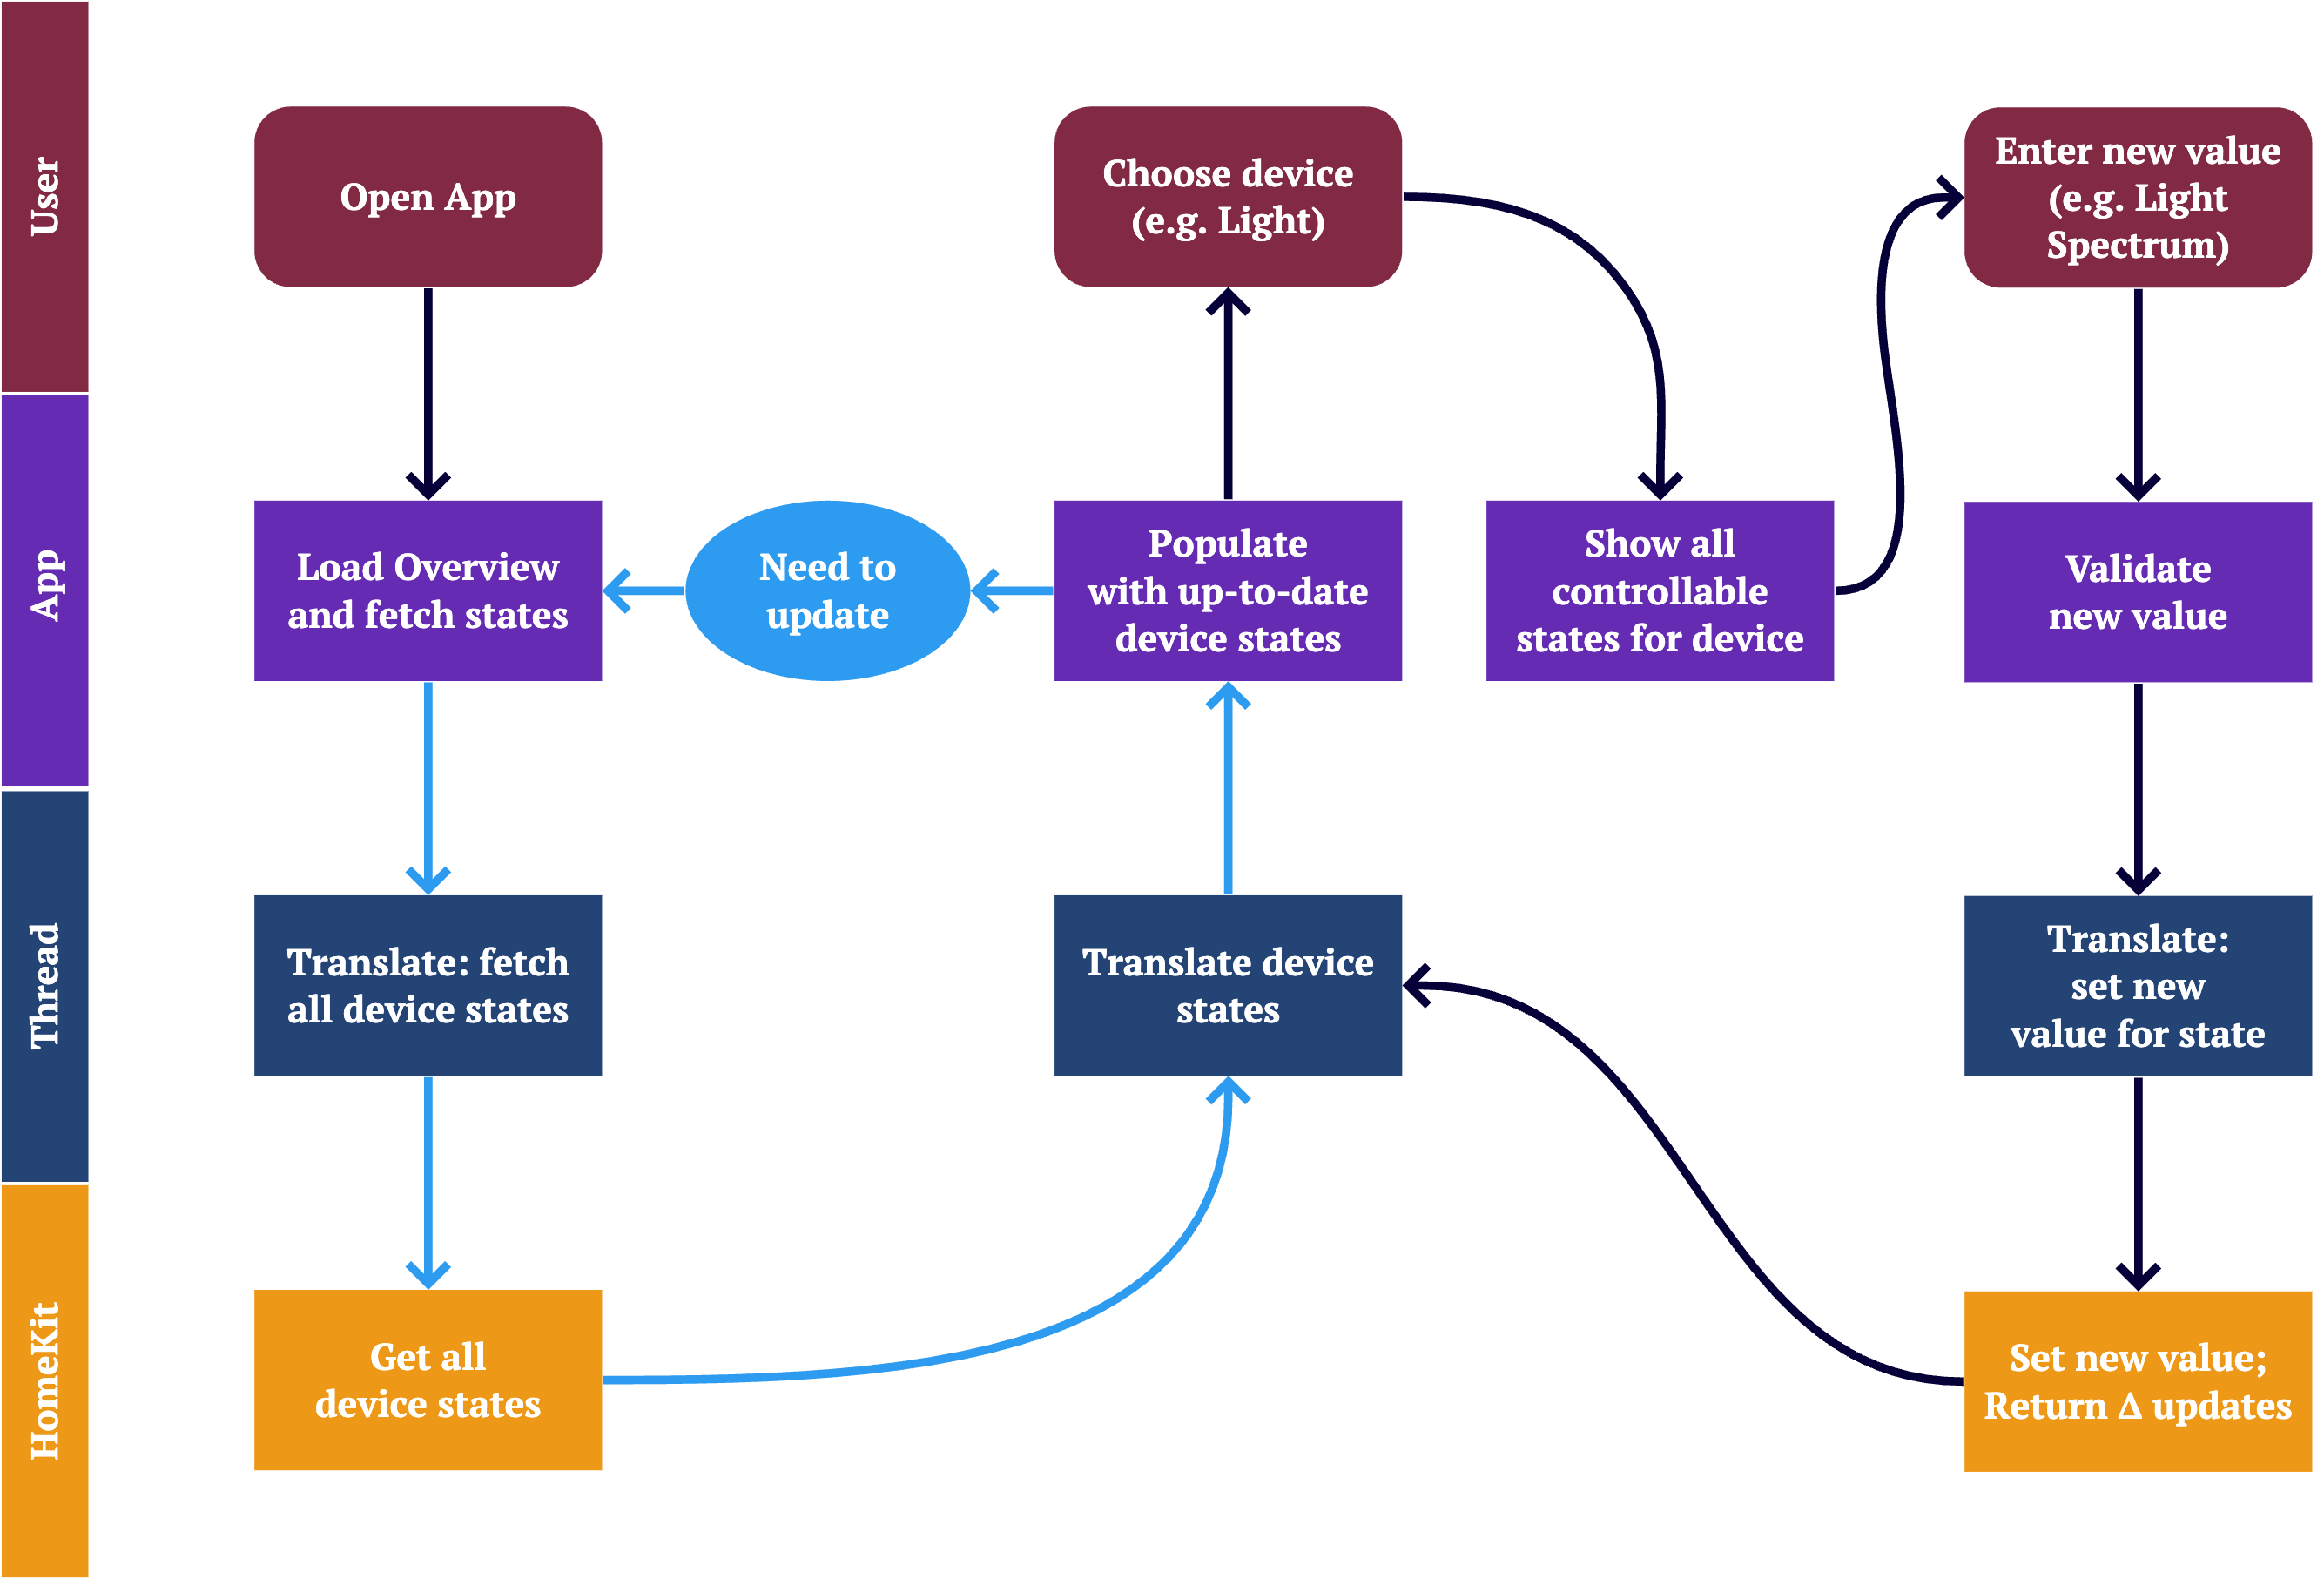
\includegraphics[width=0.9\linewidth]{data_diagram}}
    \caption{Data Architecture Diagram \label{fig:architecture_diagram}}
\end{figure}

The Platform comprises three interdependent components that complement one another. Our demo highlights two components with which users directly interact: Software, represented by the first two rows in Figure~\ref{fig:architecture_diagram}, and Hardware. The third component, Backend, comprises of an API that allows third-party hardware manufacturers to build firmware that integrates their hardware into the Platform. This API will be uploaded to GitLab \cite{codebase} at a later date.

\subsection{Software}

Through our software, users may inspect and customize the behavior of all connected devices. We created an iOS app in SwiftUI that showcases one of the most important device categories in a reef aquarium: lighting. Screenshotted in Figure~\ref{fig:diodes} is our demo app through which granular control over each group of diodes in a reef light is achieved. In this demo, we're simulating the Ecotech Radion XR30 G6 Pro reef light. For this purpose, we are primarily addressing the following 90 diodes: 4 395nm (ultraviolet), 2 405nm, 4 415nm, 12 430nm, 32 450nm, 32 465nm (blue), 2 510nm (green), and 2 645nm (red).

\subsubsection{Diode Configuration}

\begin{figure}[!htp]
    \centering
    \makebox[0pt]{%
    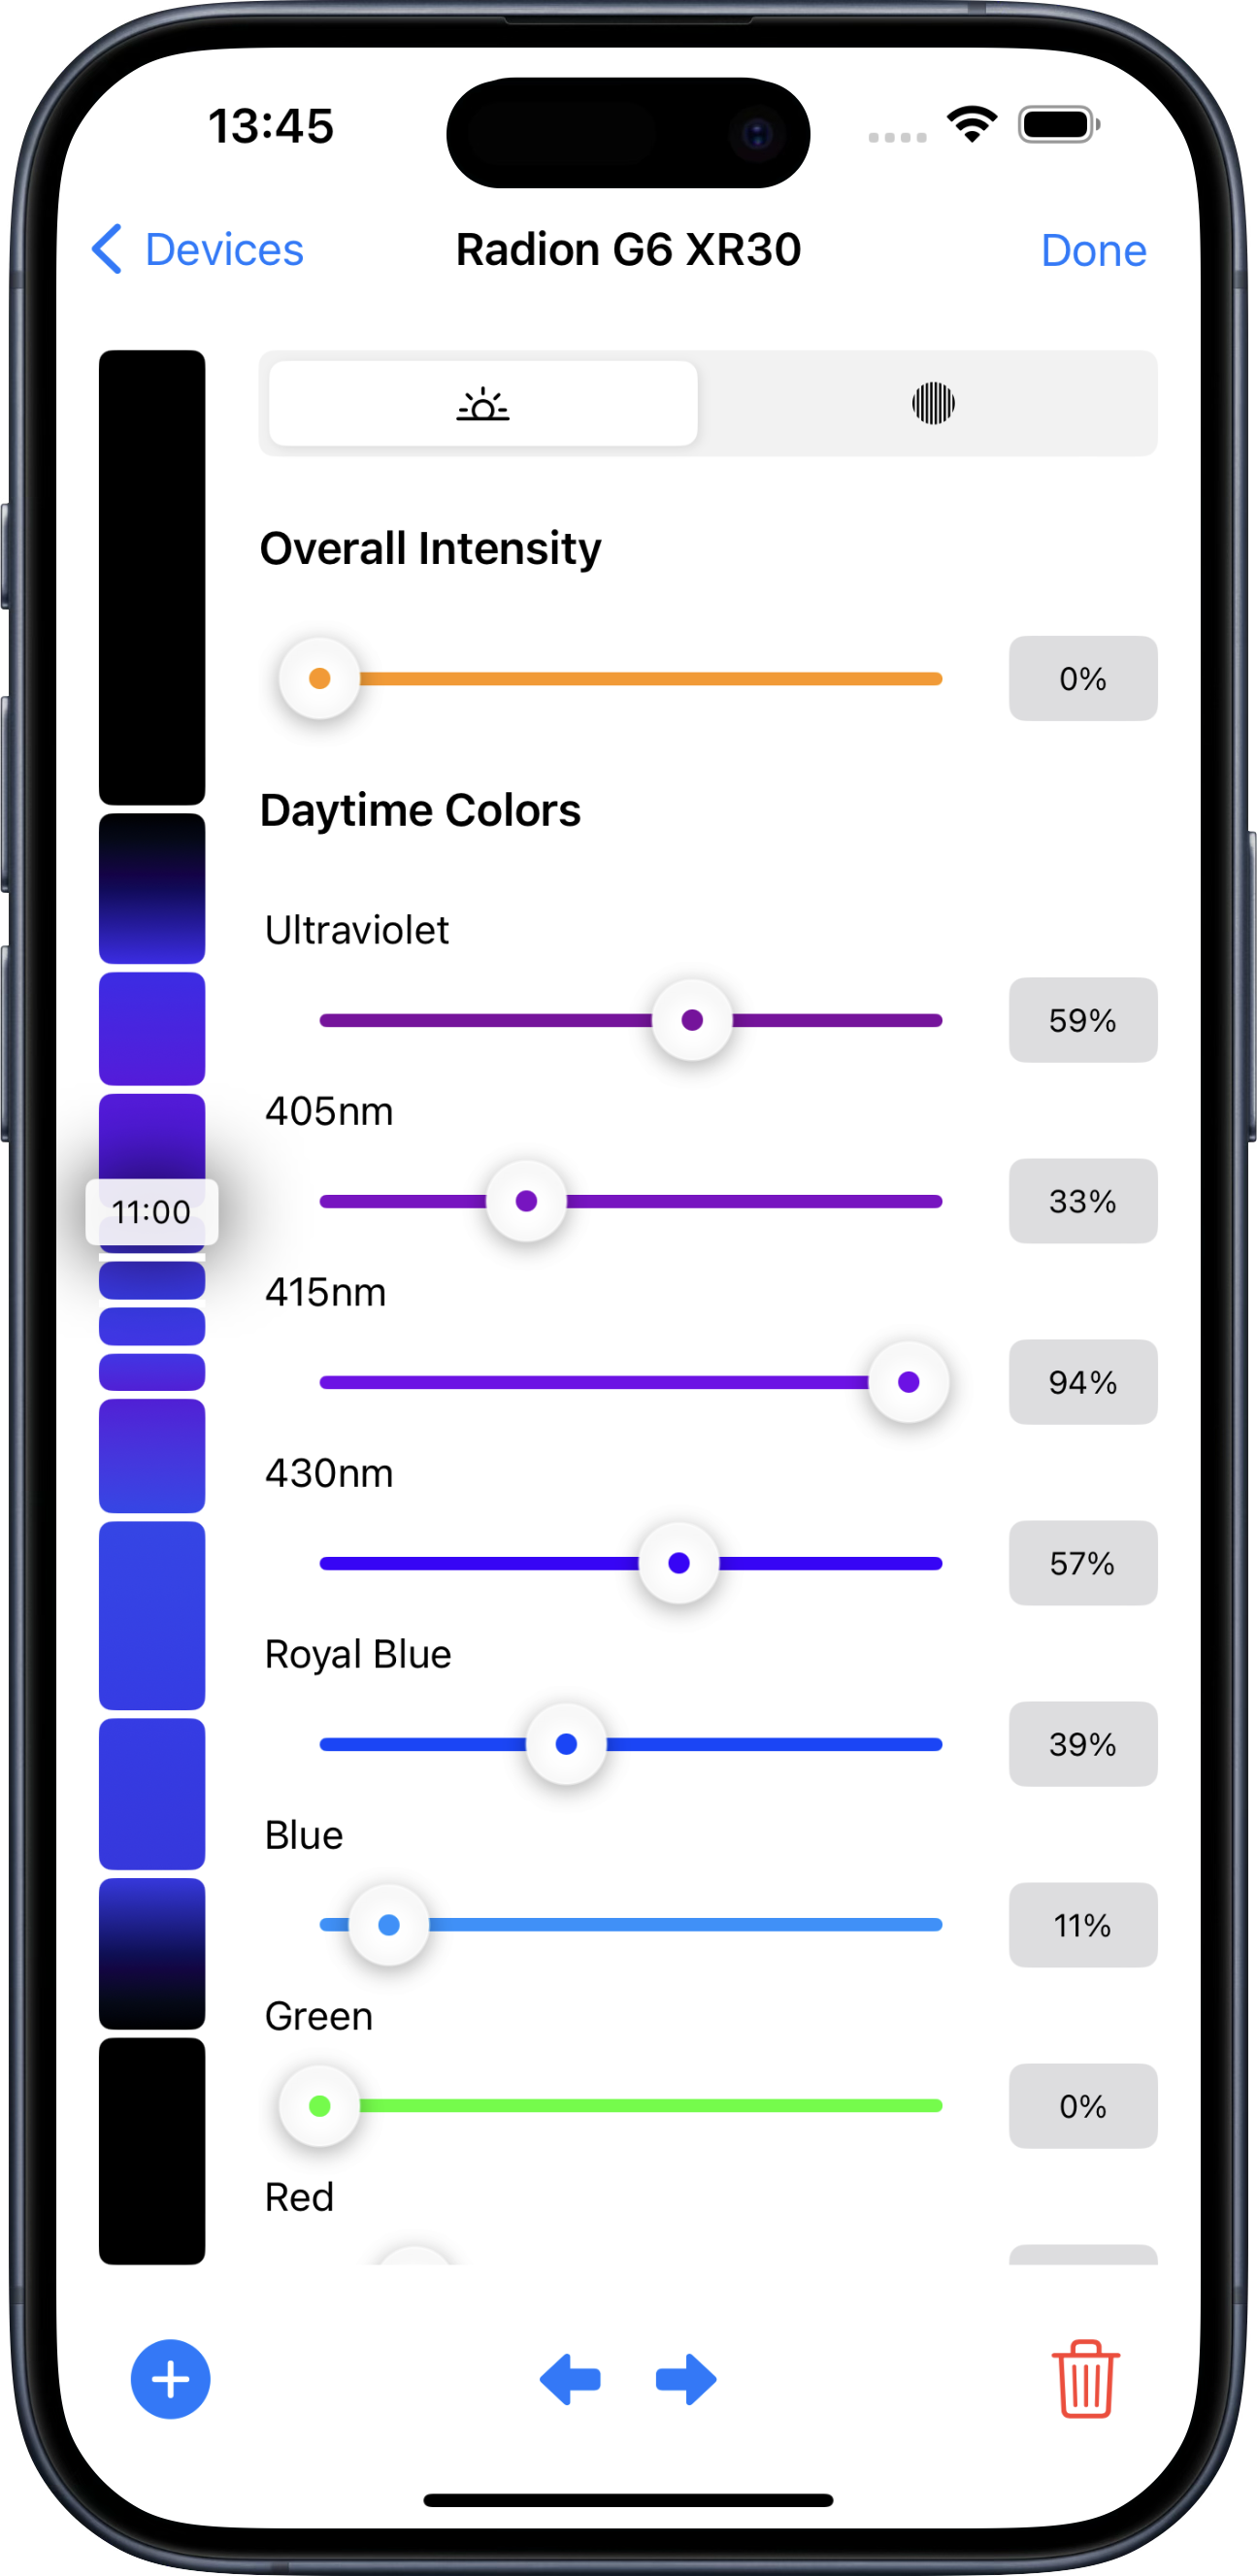
\includegraphics[height=200pt]{app_editing}}
    \caption{Diode Configuration\label{fig:diodes}}
\end{figure}

\noindent Each slider in Figure~\ref{fig:diodes} represents the intensity setting for a group of diodes emitting the same wavelength of light. For example, at intensity 39\%, all ultraviolet diodes would be set to 39\% power. We then convert all wavelengths into their approximate RGB counterparts and mix all the RGBs based on their intensity and diode count. 

\xssub{Wavelength to RGB}

\noindent While the human eye typically discerns wavelengths between approximately 400nm to 720nm, our use case incorporates extremities such as 395nm UVA, which is crucial for coral health and growth. To accommodate these variations, we define the permissible range as 380nm to 780nm.

We then map the wavelengths to their corresponding RGB values by employing a multistep formula then scaling the results so that they fall within $[0, 255]$. For example, $\lambda = 395nm$ would yield an RGB value of (92, 0, 214). The complete mapping and conversion algorithm is hosted on GitLab \cite{codebase}.


\xssub{Timeline}

\noindent On the left side of the screen, we feature a Timeline displaying breakpoints corresponding to each instance when a Diode Configuration is set. For example, Figure~\ref{fig:diodes} shows the diode configuration for the 09:30 breakpoint. The Timeline provides a dynamic visualization of the expected lighting effects throughout the day. With the gradient, users can quickly discern when the light activates or deactivates, as well as when the aquarium is expected to maximize its actinic, fluorescent glory.


\xssub{Combining RGBs}

\noindent To combine colors, we employ a simple algorithm that also takes into account the alpha, alternatively called weight, of each diode group. This means the 4 UVA/395nm diodes do not affect the combined color as much as the 32 blue/465nm diodes.

For example, to combine ultraviolet and blue, we start by converting 395nm and 465nm to their RGB values: (92, 0, 214) and (0, 178, 255). Assuming they both have an alpha/weight of 1.0, the following calculations give us a single combined color to showcase for this breakpoint on the Timeline.

\begin{align*}
	r &= (92 + 0) / 2 = 46 \\ g &= (0 + 178) / 2 = 89 \\ b &= (214 + 255) / 2 = 234
\end{align*}

\subsubsection{Spectrum Graph}

\begin{figure}[!htp]
    \centering
    \makebox[0pt]{%
    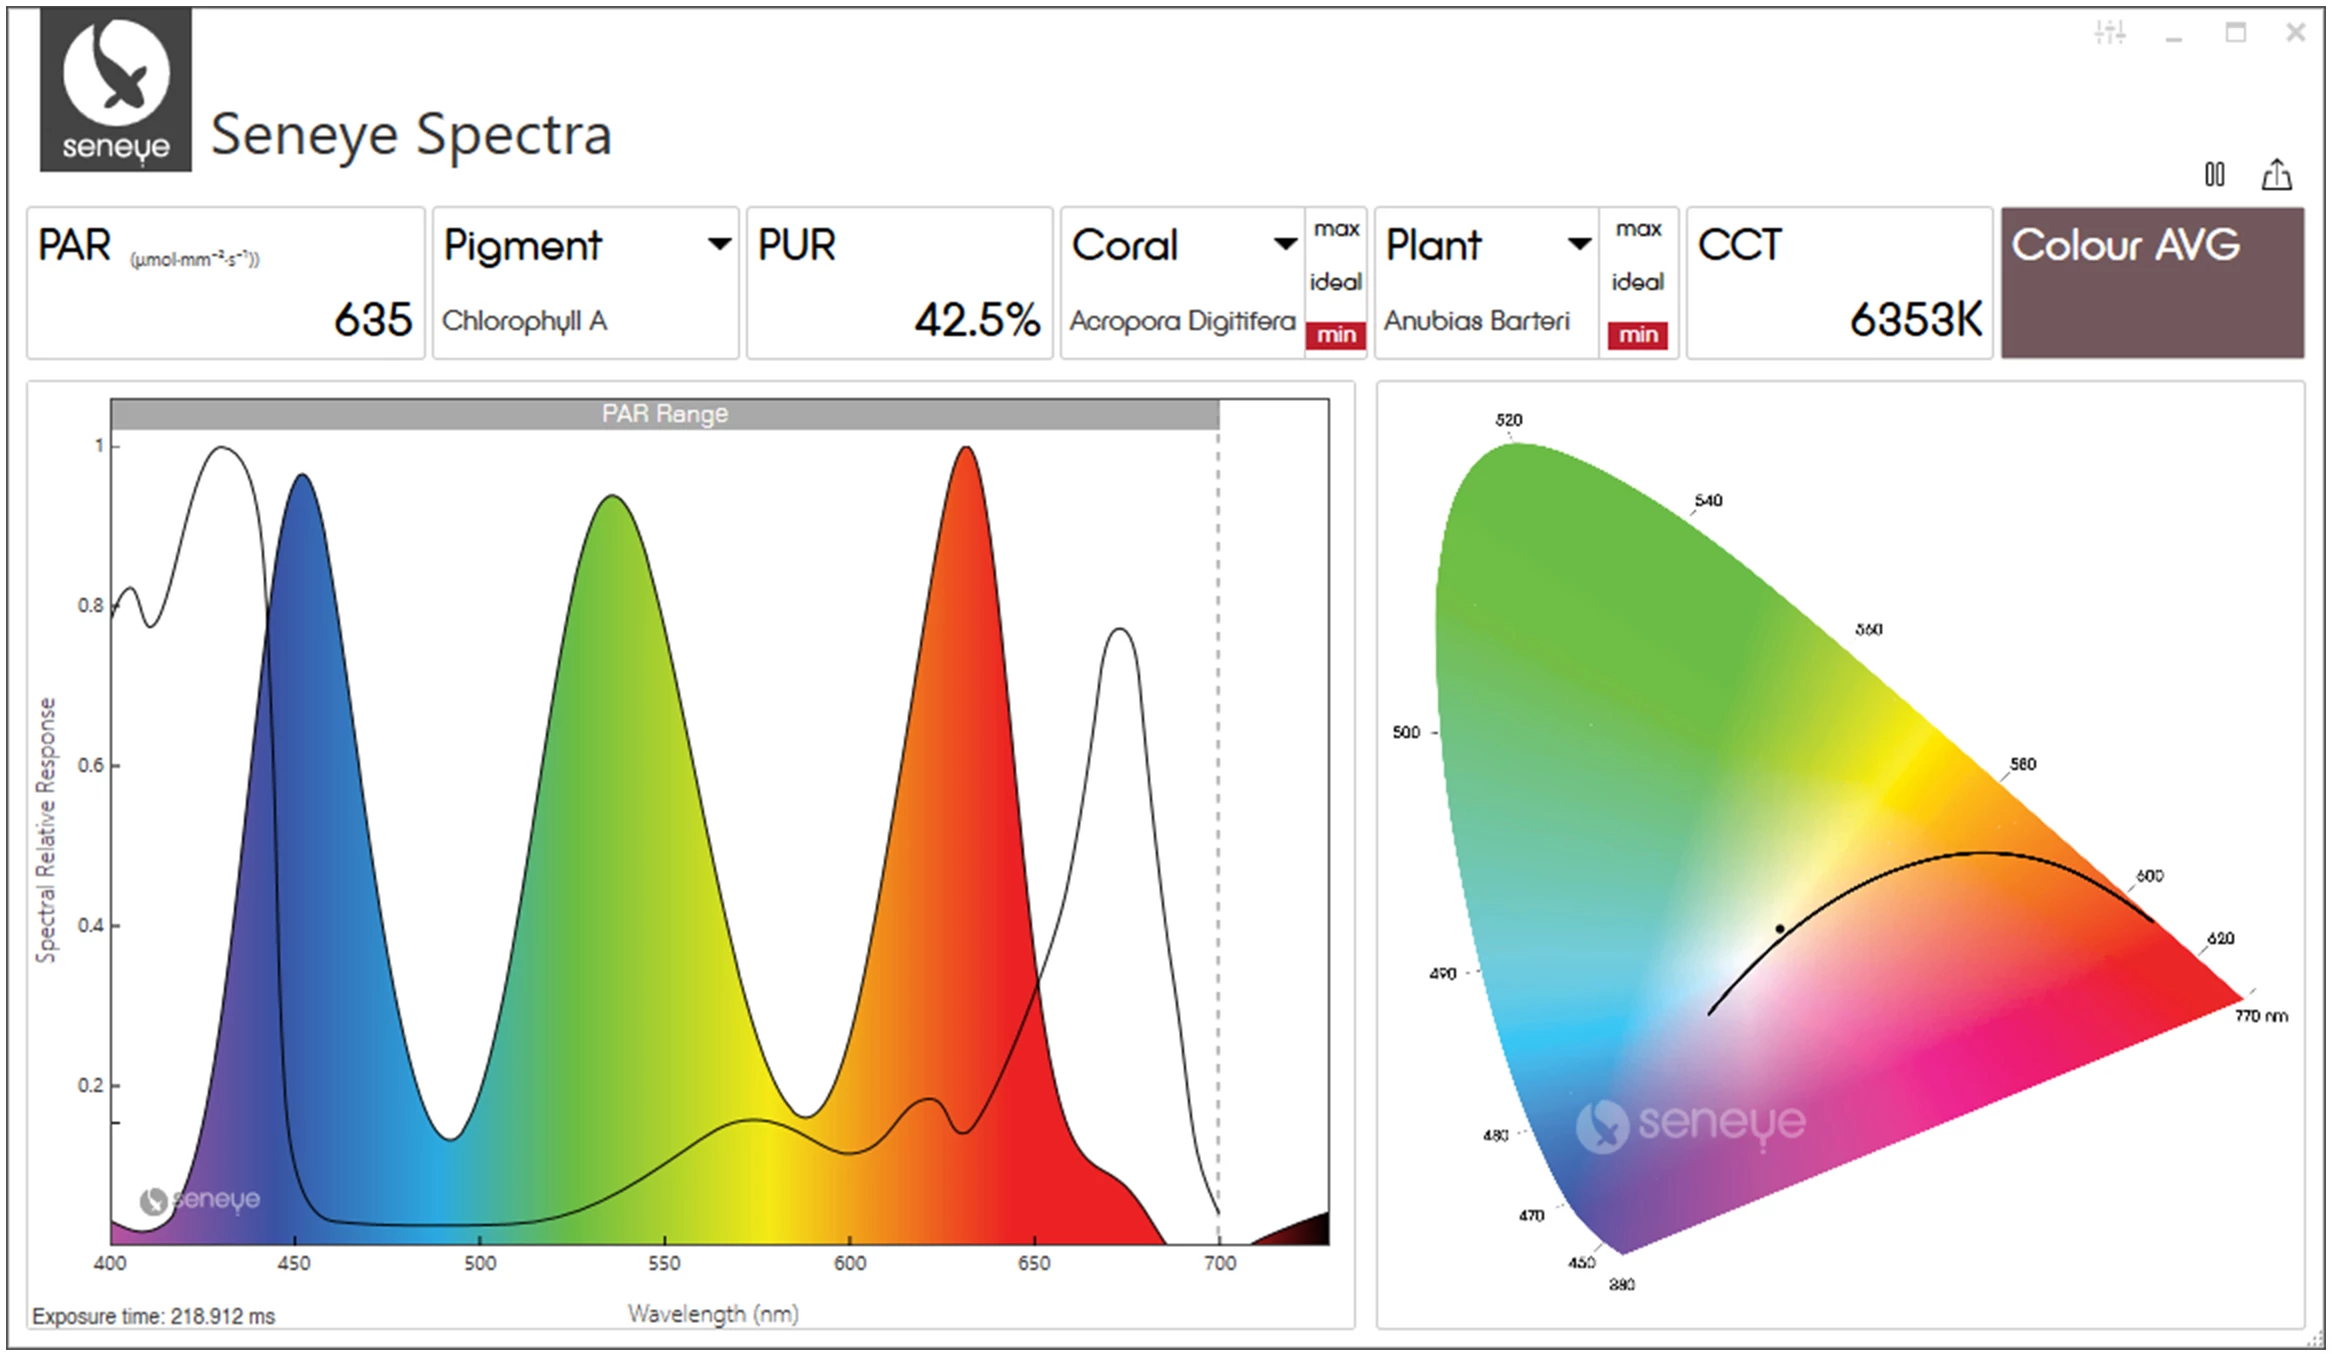
\includegraphics[width=0.9\linewidth]{seneye_spectra}}
    \caption{Seneye Spectra software on Windows\label{fig:seneye_spectra}}
\end{figure}

Professional spectrometer software typically utilizes spectrum graphs, as illustrated in Figure~\ref{fig:seneye_spectra} \cite{seneye}, to aid users in visualizing spectra within particular areas of an aquarium. Such hardware is often necessary due to the varying wavelength distributions resulting from different spatial configurations of the same multi-fixture light source. Efforts are frequently made to arrange lights to achieve the most uniform spread, as this enables aquarists to maximize the horizontal space available for coral species of similar lighting needs.

\begin{figure}[!htp]
    \centering
    \makebox[0pt]{%
    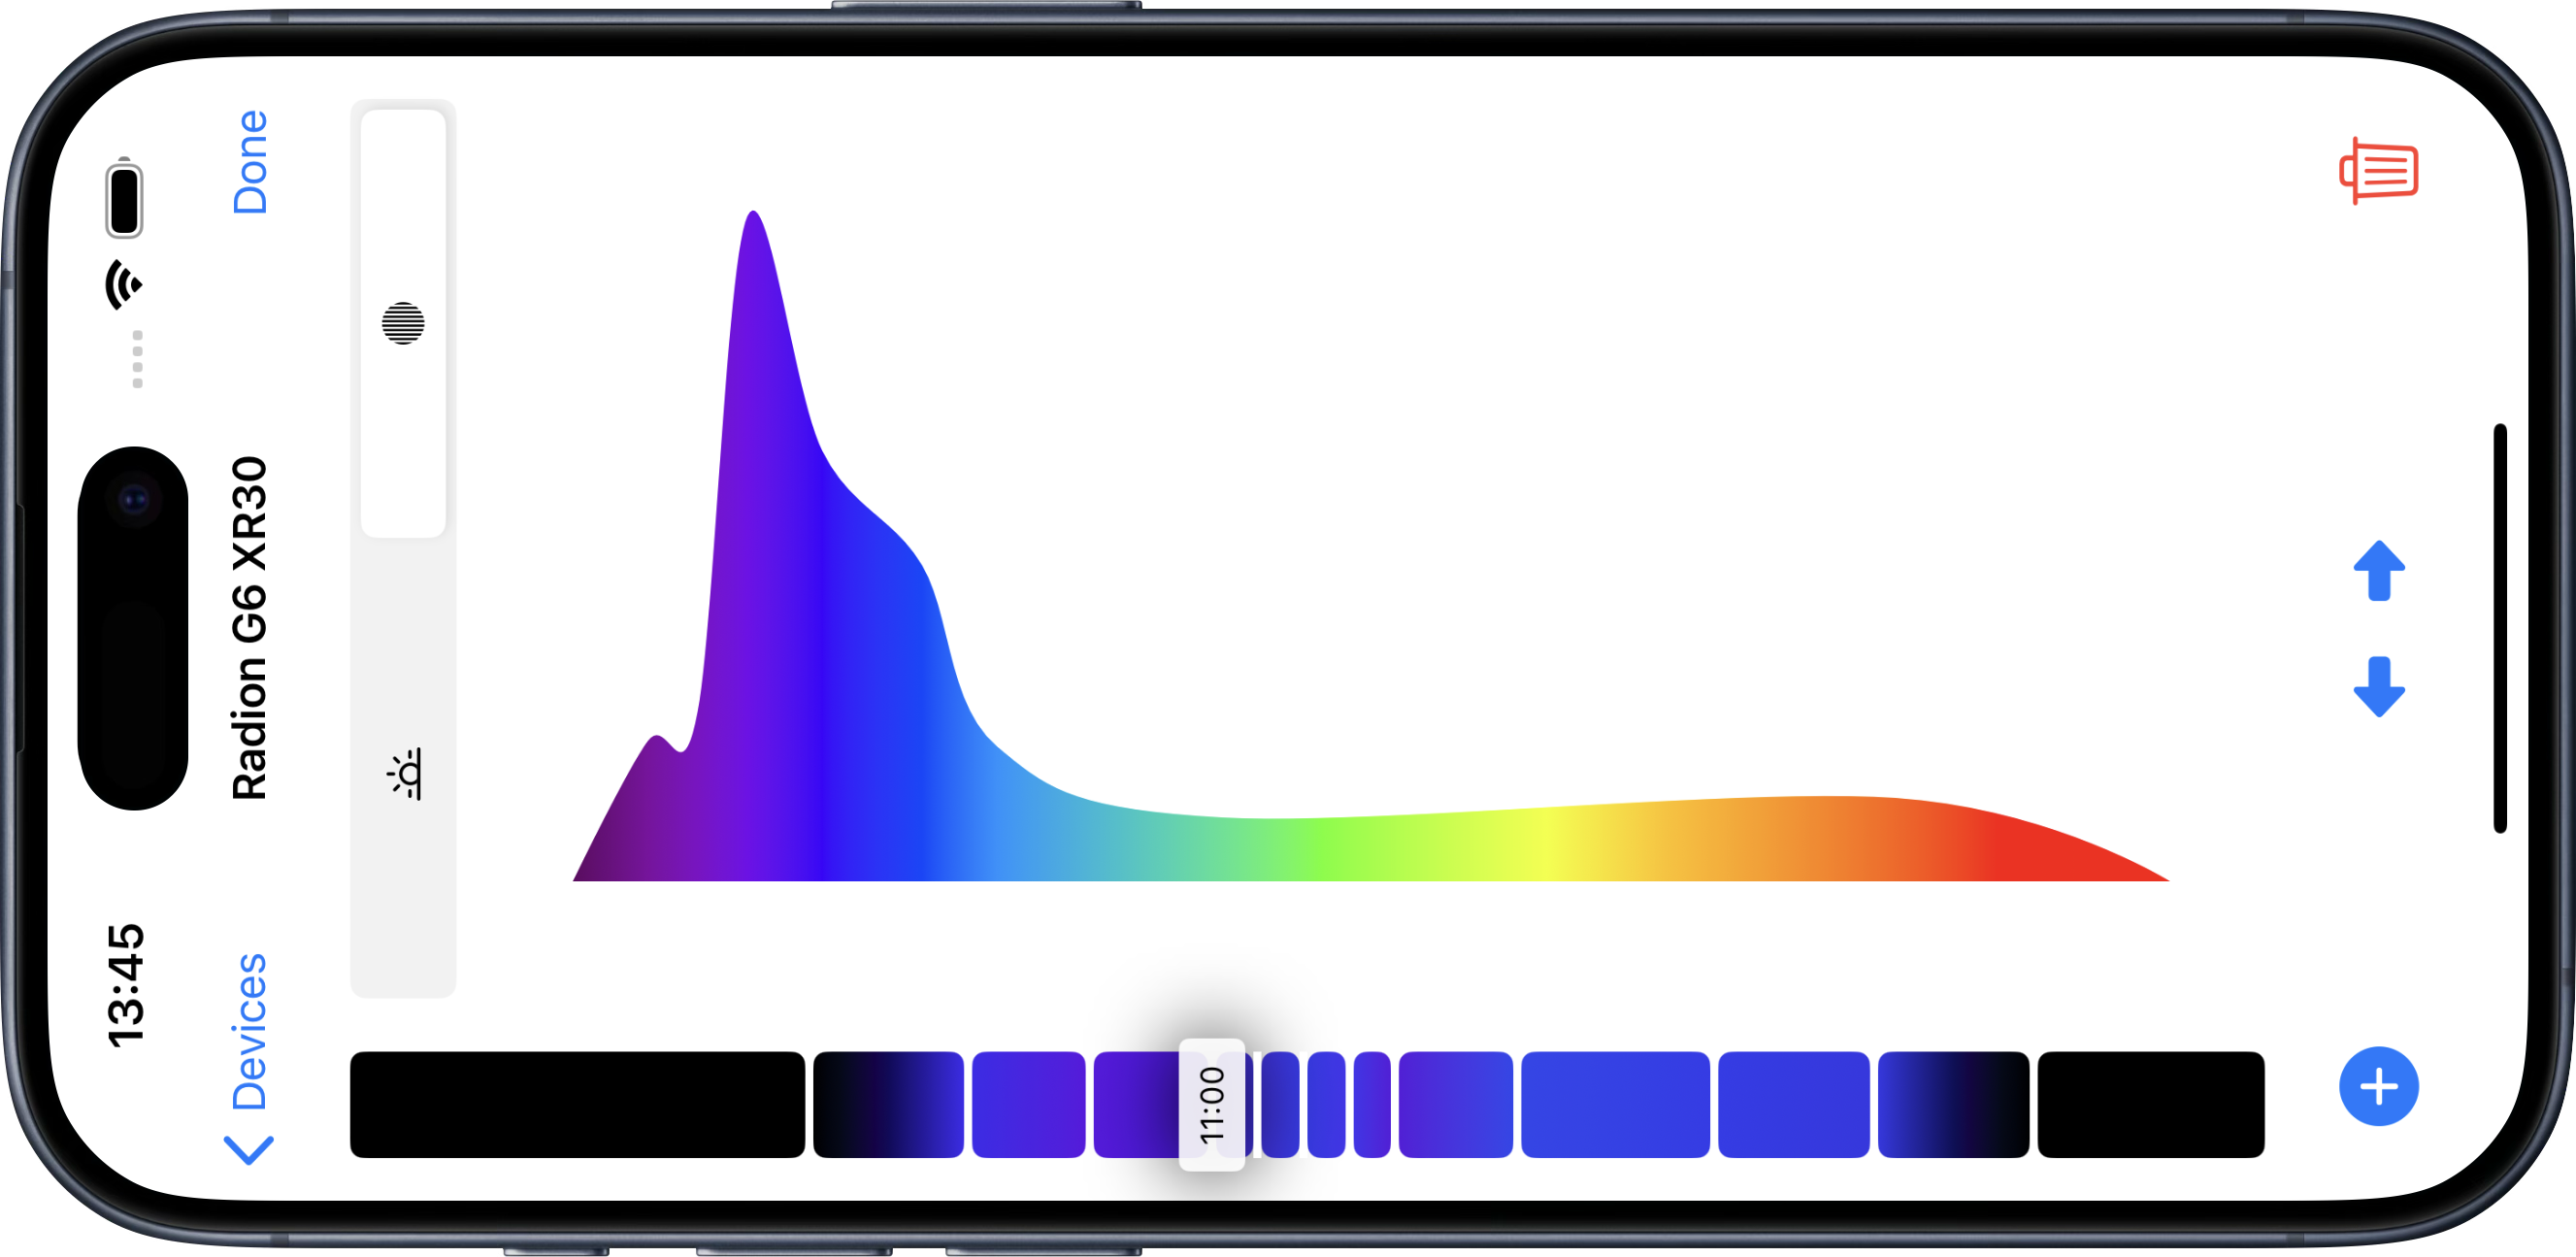
\includegraphics[width=0.9\linewidth]{app_spectrum}}
    \caption{Spectrum Graph\label{fig:spectrum}}
\end{figure}

The Spectrum Graph can be generated for any diode configurations. We congregate each diode group and plot their intensities on a 2D plane where the x-axis denotes wavelength and the y-axis denotes the weighted intensity value (see Figure~\ref{fig:spectrum}).

To draw spectra correctly, we studied multiple interpolation methods and compared their results to popular renders of spectra. We found that we could draw the most conventional spectra by using cubic spline interpolation to fill in intermediary data points. The Cubic Spline interpolation could be expressed mathematically as such:

\begin{align*}
S_i(x) &= a_i(x-x_i)^3 + b_i(x-x_i)^2 + c_i(x-x_i) + d_i \\
\end{align*}


While the Spectrum Graph is not intended to replace dedicated spectrometers for experienced reefers, we believe it offers valuable insight. Providing an estimate of the spectrum output across the effective coverage area of the light source can assist reefers in assessing the efficacy of their diode configurations. The complete interpolation algorithm is hosted on GitLab \shortcite{codebase}.


\subsection{Hardware}

We use a Beaglebone Black to showcase components of our software platform that interact and respond to the environment. The Beaglebone runs on an IoT-flavored (GUI-less) Debian OS \cite{openthread_bb}, with a photoresistor connected as per the Adafruit guide \cite{adafruit}. Our iOS app regularly retrieves data from the photoresistor, leveraging its voltage readings to assess ambient light intensity and suggest optimal diode configurations. However, this application represents just one example of the myriad uses for environmental sensors within a reef aquarium.

\xssub{Example: Temperature Sensor}

\noindent Temperature sensors play a crucial role in regulating aquatic systems, particularly in maintaining consistency within a reef aquarium. It's essential for reefers to minimize temperature fluctuations, as stability is paramount for the health of the ecosystem. Common solutions include aquarium heaters/chillers or room AC units, but such hardware are prone to failure, especially as they are often under heavy use. To mitigate this risk, reefers often implement a failsafe mechanism by integrating an additional temperature sensor into the control system. This sensor monitors ambient temperature and prompts the system to deactivate the heater/chiller if a significant deviation is detected. This often requires multiple temperature sensors for multiple pieces of hardware, and it is easy to configure incorrectly.

In our integrated Platform, no extra hardware or wiring is necessary. Users can set up Rules that respond to environmental changes automatically. For instance, if there's a notable increase in room temperature, the system triggers an alert to notify the user. The Platform can then activate backup chillers or AC units while continuously monitoring water temperature to make informed adjustments. By primarily relying on software, users are spared from dealing with excessive wiring, tinkering, and maintenance.


\subsubsection{Photoresistor}

We follow the Adafruit tutorial to correctly wire the photoresistor (Figure~\ref{fig:bb_wiring}).

\begin{figure}[!htp]
    \centering
    \makebox[0pt]{%
    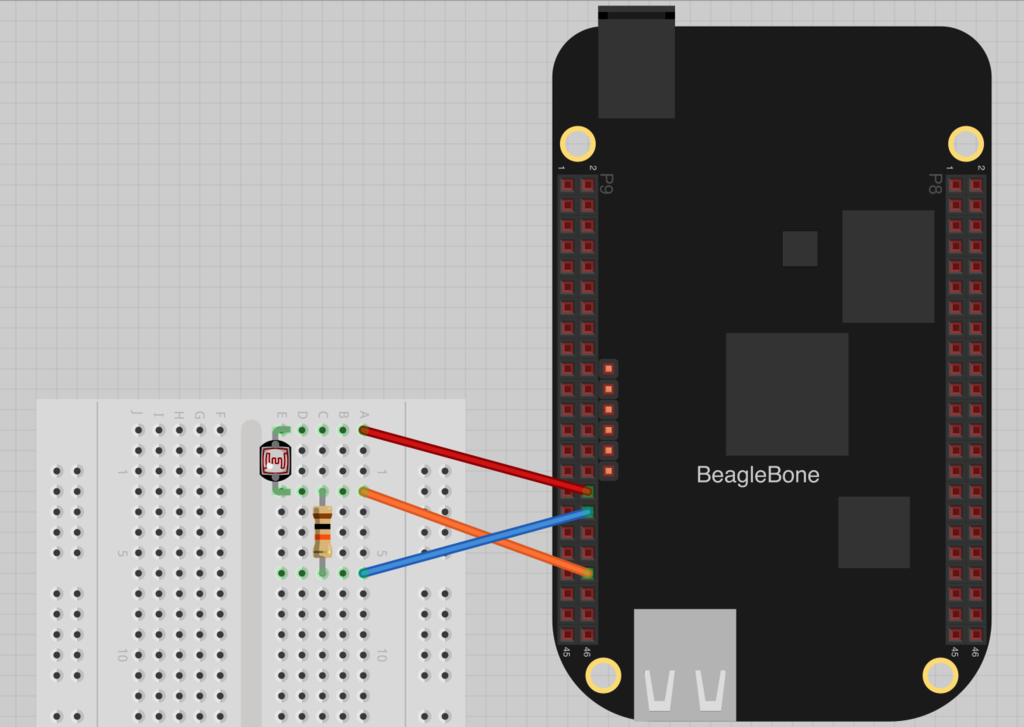
\includegraphics[width=0.9\linewidth]{beaglebone_fritzing}}
\end{figure}
\begin{figure}[!htp]
    \centering
    \makebox[0pt]{%
    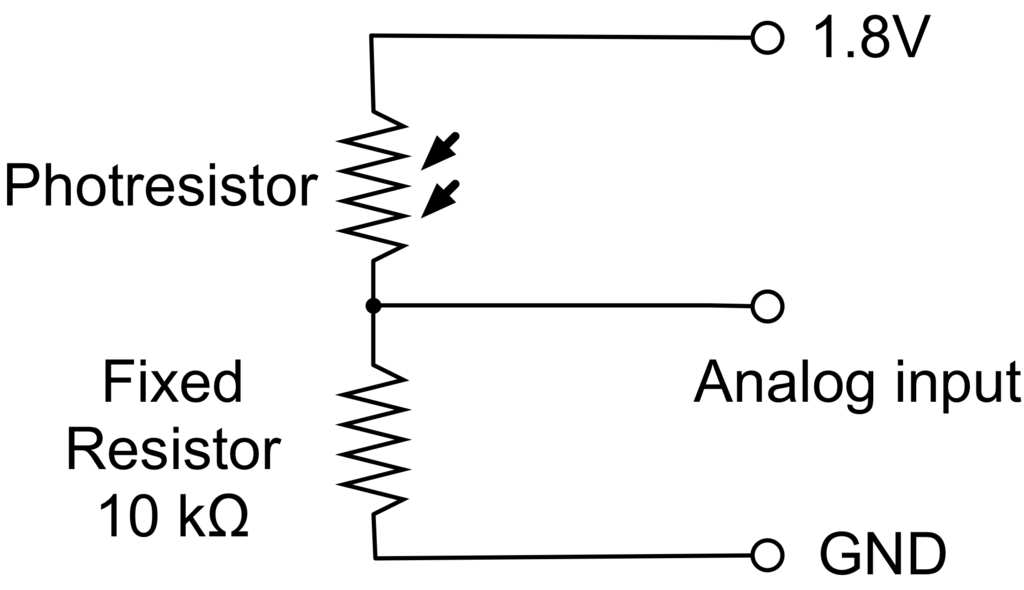
\includegraphics[width=0.9\linewidth]{beaglebone_voltage_divider}}
    \caption{Beaglebone Wiring}
    \label{fig:bb_wiring}
\end{figure}


Reading from the photoresistor is simple. The \texttt{Adafruit\_BBIO} library enables access to the GPIO pins on the Beaglebone, acquiring sensor outputs that can be roughly converted to voltage using the following formula:

\begin{align*}
	volts = reading * 1.800
\end{align*}

The iOS app begins by guiding users to move the sensor inside and around the aquarium to establish a baseline reading of the system. It records this initial reading and can use it as a reference for future spectrum recommendations. Once initialized, whenever reading mode is engaged, the app fetches readings every few seconds and proposes adjustments to diode intensity. The app is also primed to take advantage of more advanced light sensors that provide more precise lumen or PAR data to enable spectrum customizations, should users opt to incorporate additional sensors.

\subsubsection{Website}

\begin{figure}[!htp]
    \centering
    \makebox[0pt]{%
    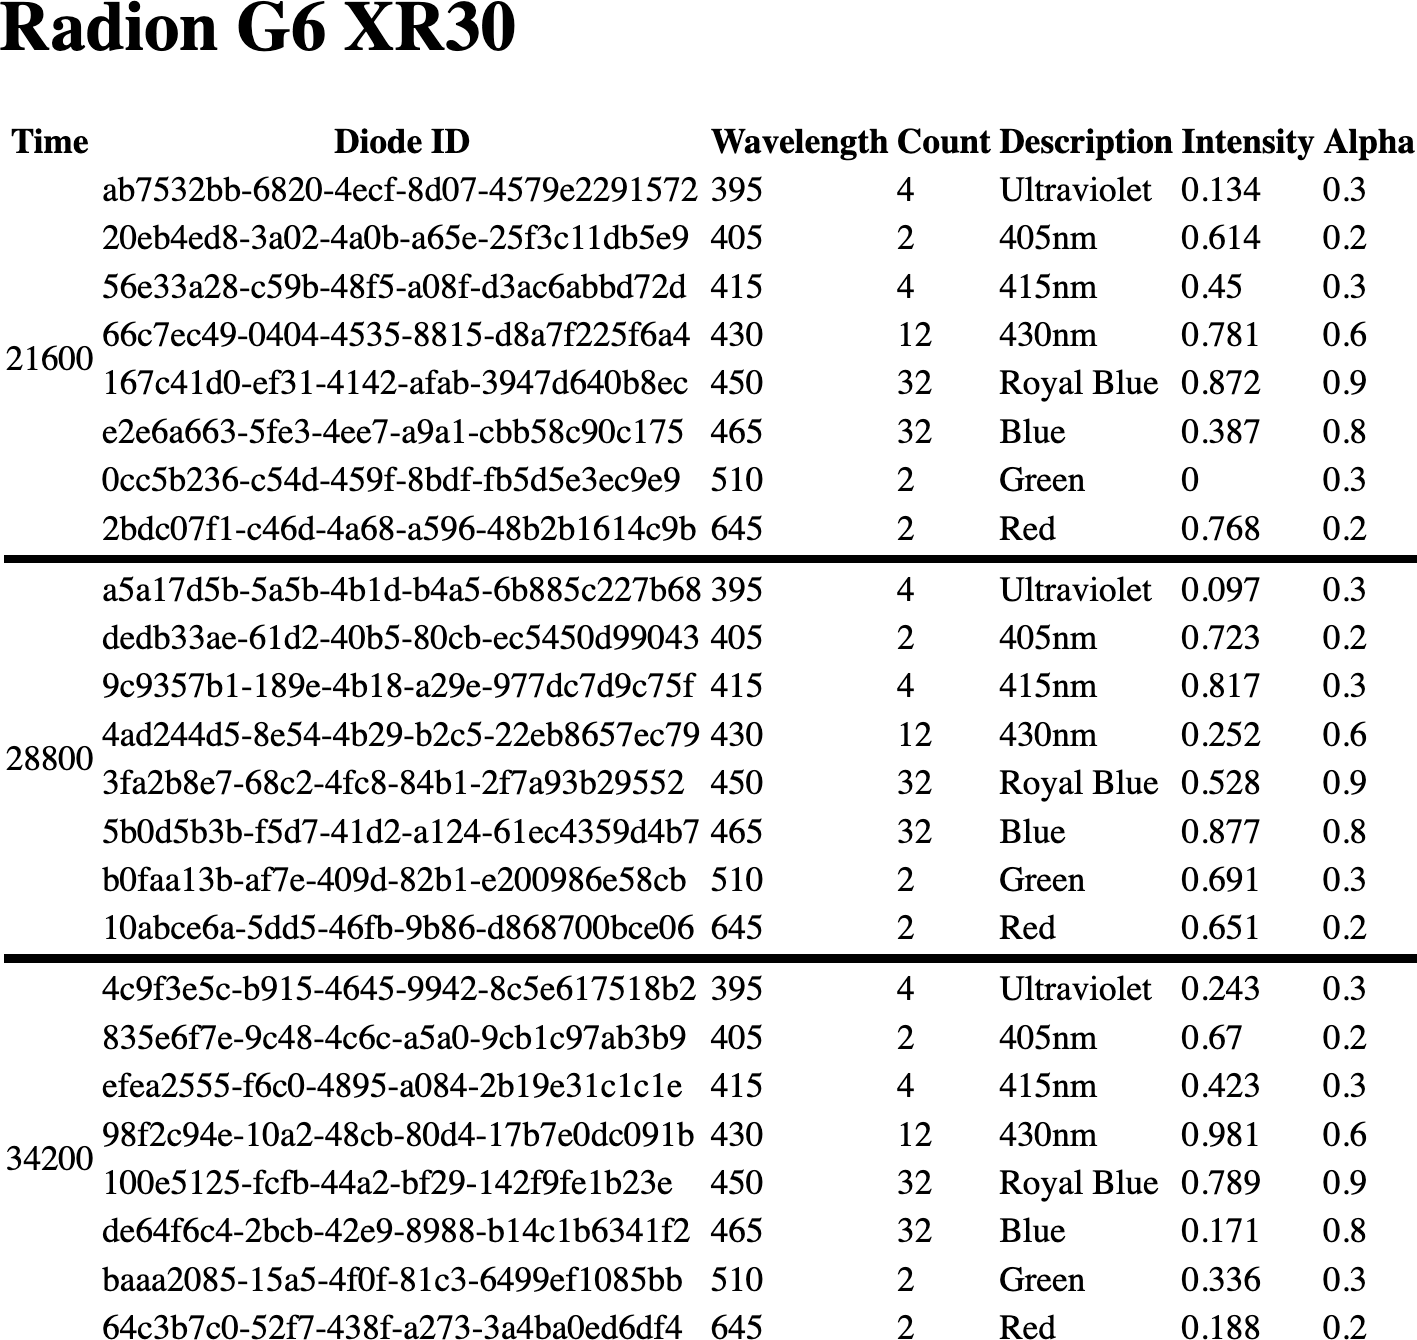
\includegraphics[width=0.9\linewidth]{beaglebone_server}}
    \caption{Beaglebone Server}
    \label{fig:bb_server}
\end{figure}

The Beaglebone hosts a server through Flask/Python. The server's homepage displays the current diode configuration of the device (Figure~\ref{fig:bb_server}) and has three routes. The first two routes, \texttt{get\_data} and \texttt{update\_data}, allow the iOS app to read and update diode configurations. The third route, \texttt{get\_reading}, shares the photoresistor's output with our software. After enabling Internet Sharing with the Beaglebone\footnote{On macOS, enable Networking Sharing with the USB-connected Beaglebone, then run \texttt{sudo dhclient eth0} to enable internet \cite{bb_internet}}, we can access the server at \url{beaglebone.local:8080}. Future firmware versions to enable more functionalities should still follow the same three-route principle.


\section{Conclusion}

Through our software/hardware demo, we illustrate the journey of a hobbyist embarking on the setup of their aquarium. With the aid of an integrated smart system, the hobbyist navigates the initial setup phase with confidence, sidestepping potential pitfalls that could disrupt the delicate balance of their burgeoning aquatic ecosystem. Real-time sensor data empower users to make informed decisions, enabling them to make timely adjustments and optimize conditions for aquatic life.

As the system accumulates data over time, it evolves to be capable of autonomously managing various aspects of aquarium maintenance. This autonomy not only streamlines the caretaking process but also grants hobbyists the freedom to delve deeper into the mesmerizing intricacies of marine life.

Expanding this out to research to allow for more efficient reef studies in labs
Automation allows for better biological studies
Intricacies of marine life


\section{Future Work}

Potential enhancements could involve expanding the range of hardware categories supported, including wavemakers, peristaltic dosers, etc.

To fully showcase the advantages of OpenThread over alternative connectivity standards, additional hardware are necessary. For example, by incorporating a broader array of sensors, we can better highlight the capabilities of OpenThread within our integrated aquatic control system.

We hope to expand the project scope to enable more research on marine life. Autocollection of environment data 

\section{Acknowledgements}

I would like to thank the esteemed faculty of the Computer Science department at Earlham College and friends who have supported me. Specifically, I want to thank Dr. Charlie Peck for his hardware expertise and general guidance, Dr. David Barbella for his feedback on my ideas and research proposal, Porter Libby for his help in brainstorming effective implementations of those ideas, and Gary Coker for proofreading and thoughtful discussions when bouncing ideas around.

\bibliographystyle{apacite}
\bibliography{references}


\end{document}
